\chapter{SUPPLEMENTAL MATERIAL FOR CHAPTER V}

\section{Supplemental Figures}
This section includes the supplemental figures referenced in chapter V. Other supplemental files such as spreadsheets, newick trees, and multiple sequence alignments are included in the chapter 5 sub--directory of the zipped supplemental directory submitted with this dissertation.

\begin{figure}
\centering
	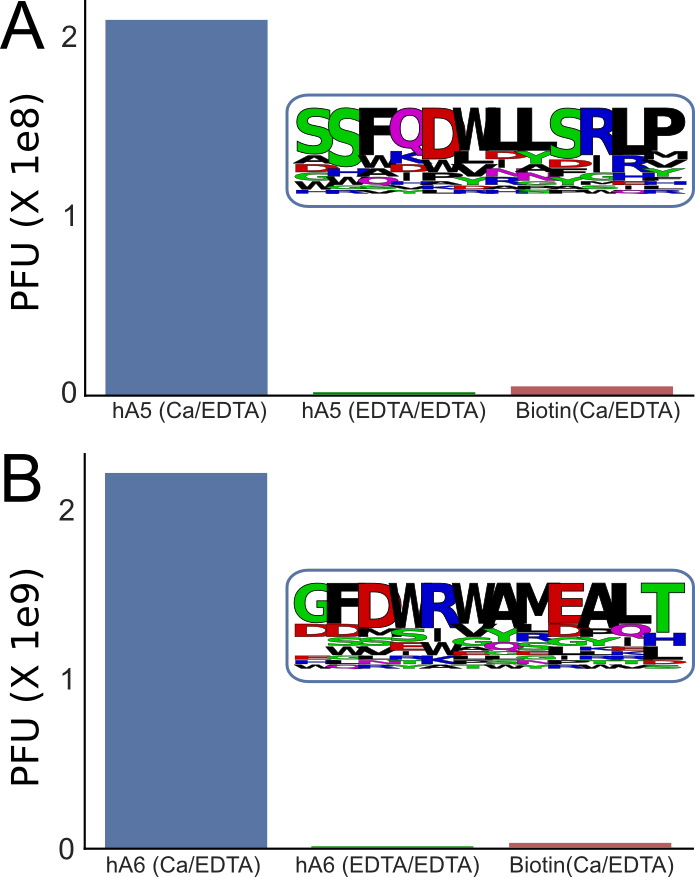
\includegraphics{ch5-figS1.png} 
\caption[Randomer phage enrichment is dependent on Ca\textsuperscript{\textbf{2+}}
and protein]{Randomer phage enrichment is dependent on Ca\textsuperscript{\textbf{2+}}
and protein. Bar graphs show the plaque forming units (PFU) for phage
solutions after the third round of enrichment for screens using hA5
(A) or hA6 (B). For each round of panning, we incubated phage with
biotinylated protein, pulled down bound phage via a streptavidin plate,
and finally eluted the phage from the protein with an elution buffer.
To verify that binding occurred in a $Ca^{2+}$-dependent manner,
we compared $Ca^{+}$-loading/$EDTA$-elution to $EDTA$-loading/$EDTA$-elution.
We also performed a $Ca^{2+}$-loading/$EDTA$-elution experiment
using biotin alone. Insets show sequence logos (WebLogo) generated
from 20 plaque sequences from each $Ca^{2+}/EDTA$ panning experiment.
The most frequent residue at each position was used to generate the
A5cons and A6cons peptides.\label{samplefigure}}	
\end{figure}


\begin{figure}
\centering
	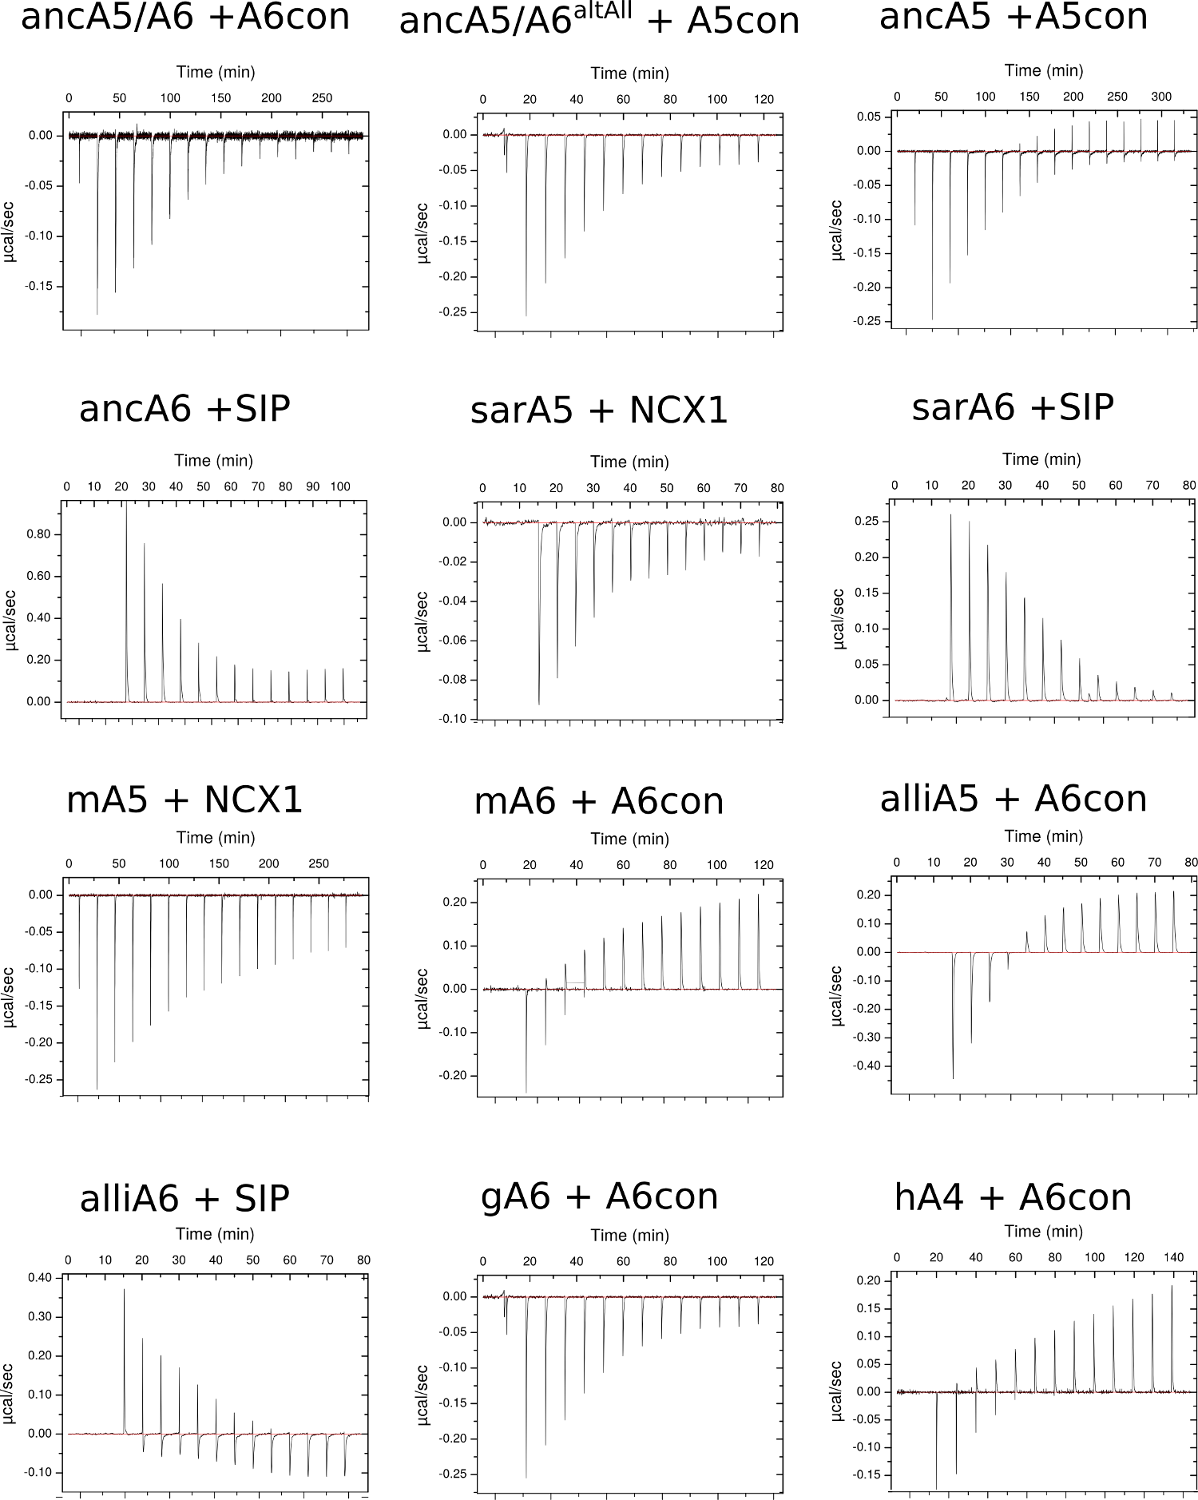
\includegraphics{ch5-figS2.png} 
\caption[Representative raw ITC data traces for each protein]{ITC traces show baseline-corrected titration of various
peptides onto S100 proteins in the presence of $2\ mM\ Ca^{2+}$.
All experiments were done with $\approx$ 100 $\mu M$ protein in $25\ mM$
TES, $100\ mM$ NaCl, $1\ mM\ TCEP$ at $pH\ 7.4$, $25\ ^{\circ}C$.CD spectra are mapped onto a diagram of the S100A5-S100A6
clade. Curves are spectra of apo (gray) and Ca\textsuperscript{2+}–bound
(orange/purple) proteins. The S100A5 proteins (purple) are characterized
by a deep alpha-helical signal at 222nm that substantially increases
in response to binding of Ca\textsuperscript{2+}. S100A6 proteins
(orange) show comparatively minimal response and maintain a deeper
peak at 208nm. These patterns hold for the ancestors at the base of
each clade. The spectra of ancA5/A6 and the ancA5/A6 altAll version
(both shown in green) resemble that of an extant S100A6, indicating
that the large Ca\textsuperscript{2+}-driven conformational change
seen in the extant S100A5s is a derived feature of this lineage.\label{samplefigure}}	
\end{figure}


\begin{figure}
\centering
	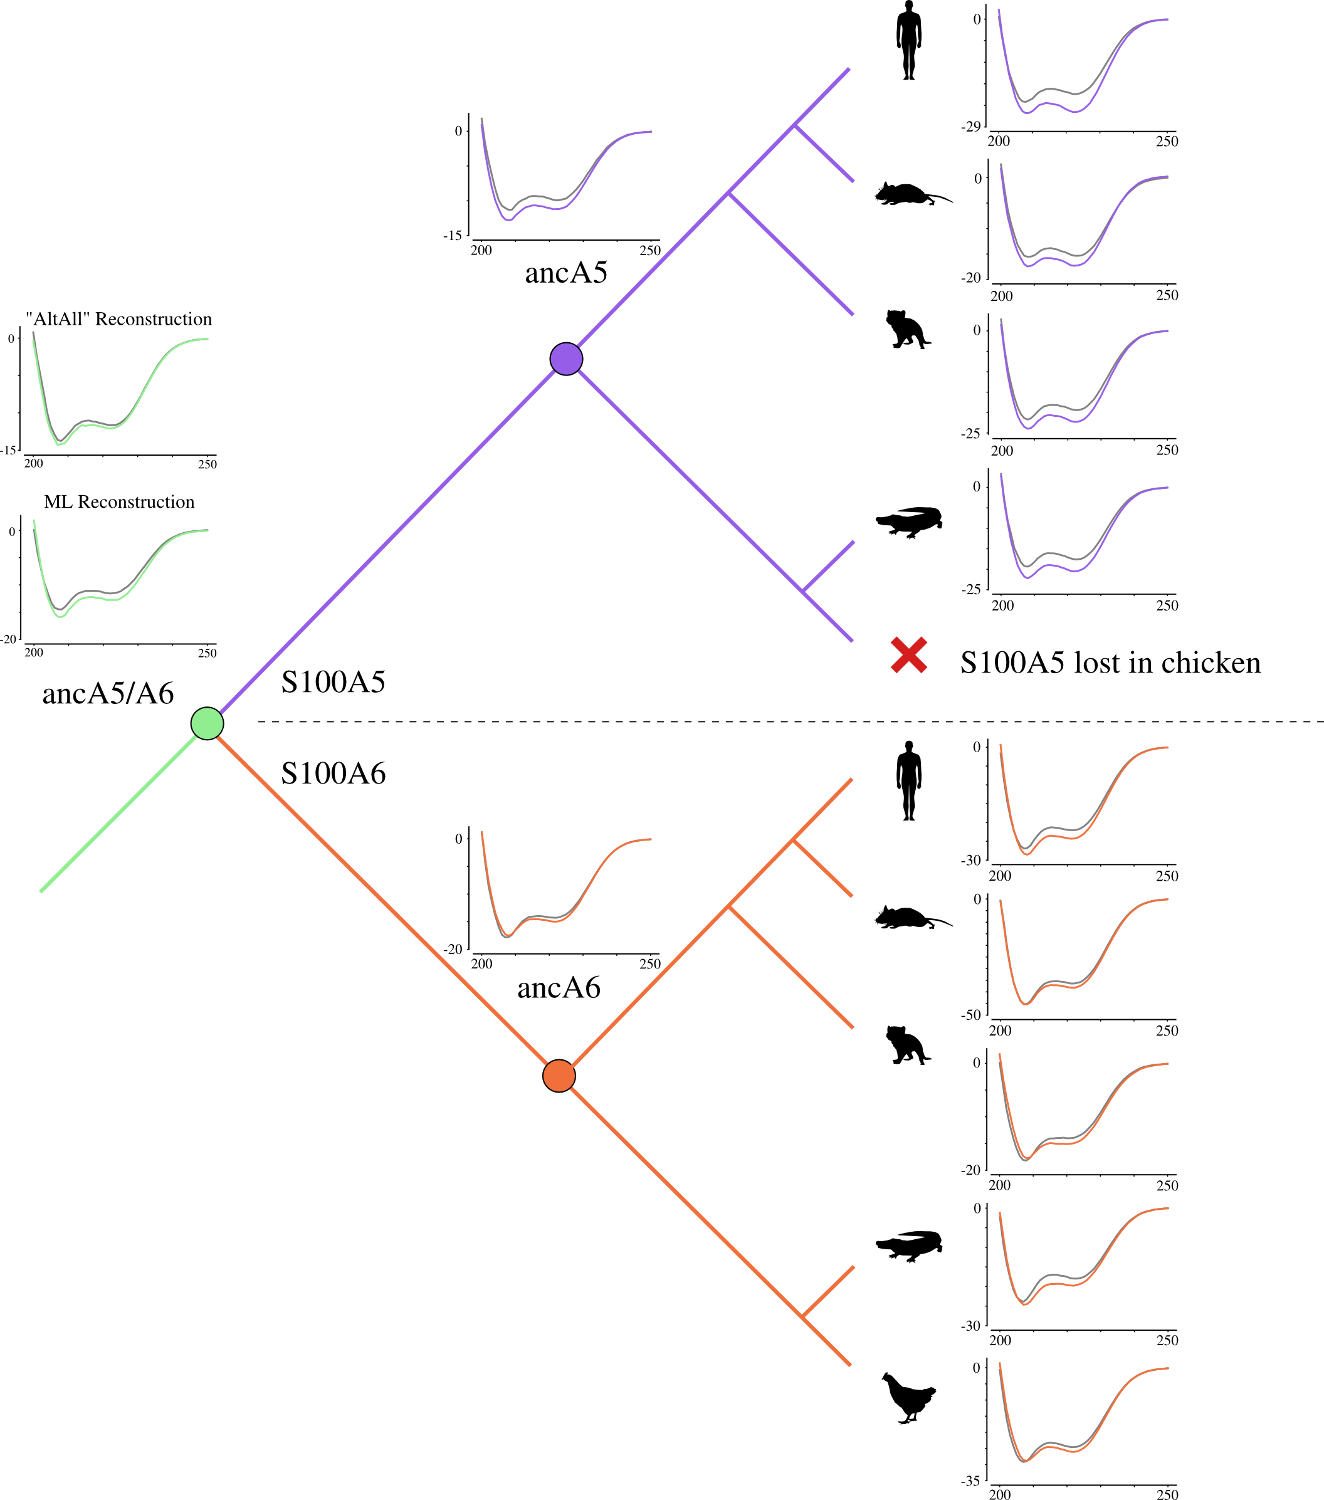
\includegraphics{ch5-figS3.png} 
\caption[Far UV CD spectra are diagnostic for S100A5 and
S100A6]{Far UV CD spectra are diagnostic for the S100A5 and
S100A6 clades. CD spectra are mapped onto a diagram of the S100A5-S100A6
clade. Curves are spectra of apo (gray) and Ca\textsuperscript{2+}–bound
(orange/purple) proteins. The S100A5 proteins (purple) are characterized
by a deep alpha-helical signal at 222nm that substantially increases
in response to binding of Ca\textsuperscript{2+}. S100A6 proteins
(orange) show comparatively minimal response and maintain a deeper
peak at 208nm. These patterns hold for the ancestors at the base of
each clade. The spectra of ancA5/A6 and the ancA5/A6 altAll version
(both shown in green) resemble that of an extant S100A6, indicating
that the large Ca\textsuperscript{2+}-driven conformational change
seen in the extant S100A5s is a derived feature of this lineage. \label{samplefigure}}	
\end{figure}


\begin{table}[h!]\footnotesize
\centering
\caption[Binding of 12-mer phage display peptides
does not depend\newline on solubilizing flanks] {Binding of 12-mer phage display peptides
does not depend on solubilizing flanks. List of phage display consensus
peptides used in the study. The sequences of flank variants of A5cons
and A6cons are shown. Flanks are indicated by lower-case letters.
The third column shows dissociation constants for peptides binding
to hA5 with 95\% credibility regions from Bayesian fits of one ITC
dataset per variant. Flank variants bind with similar $K_{D}$.}


\begin{tabular}{ccc}
Peptide Name & Amino Acid Sequence & $K_{D}$($\mu M$)\tabularnewline
\hline 
A5cons (variant 1) & \texttt{rshsSSFQDWLLSRLPgggsae} & $4.9\le6.1\le7.8$\tabularnewline
A5cons (variant 2) & \texttt{-{}-{}-{}-SSFQDWLLSRLP-ggsae} & $1.1\le2.8\le7.9$\tabularnewline
A5cons (variant 3) & \texttt{rshsSSFQDWLLSRLP-{}-{}-{}-{}-{}-} & $7.2\le9.6\le13.1$\tabularnewline
A6cons (variant 1) & \texttt{rshsGFDWRWGMEALTgggsae} & $0.3\le0.9\le2.4$\tabularnewline
A6cons (variant 2) & \texttt{-{}-{}-{}-GFDWRWGMEALT-ggsae} & $1.5\le2.5\le4.0$\tabularnewline
\end{tabular} 
\end{table}




\begin{table}[h!]\footnotesize
\centering
\caption[Parameters for binding of A6cons to S100A5 and S100A6] {Thermodynamic parameters for binding of the peptide
rshsGFDWRWAMEALTggsae (A6cons) to S100A5 and S100A6 proteins.Species
abbreviations are ``alli'' (alligator), ``gal'' (chicken), ``sar''
(tasmanian devil), ``m'' (mouse), and ``h'' (human). Fit parameters,
with standard deviation from fits, for  to the data shown schematically
in Fig 4A. Parameters are for a single-site binding model. ``NA''
indicates that there was no detectable binding. We floated the fraction
competent parameter to capture uncertainty in peptide and protein
concentration, particularly given the low extinction coefficients
of S100A5 and S100A6. If an experiment was done at both $10$ and
$25\ ^{\circ}C$, the parameters correspond to the $10\ ^{\circ}C$
experiment.}
\begin{tabular}{cccccc}
protein & $K_{A}\ (M^{-1})$ & $\Delta H^{\circ}\ (kcal/mol)$  & $fx\ comp.$ & $num\ reps$ & $T\ (^{\circ}C)$\tabularnewline
\hline 
ancA5/A6 & $8.30e5\pm1.9e5$ & $-12.20\pm1.2$ & $0.70\pm0.02$ & 2 & 25\tabularnewline
altAll & $1.10e5\pm5.2e4$ & $-8.70\pm0.6$ & $0.90\pm0.07$ & 2 & 25\tabularnewline
\hline 
ancA5 & $7.70e5\pm2.1e5$ & $-3.30\pm0.8$ & $0.80\pm0.07$ & 2 & 25\tabularnewline
alliA5 & $4.40e5\pm6.8e4$ & $-10.60\pm0.7$ & $0.70\pm0.01$ & 2 & 25\tabularnewline
sarA5 & $2.50e5\pm1.6e5$ & $-5.90\pm2.5$ & $0.90\pm0.13$ & 2 & 25\tabularnewline
mA5 & $2.10e5\pm5.4e4$ & $-11.70\pm2.7$ & $1.10\pm0.05$ & 2 & 25\tabularnewline
hA5 & $4.10e5\pm9.8e4$ & $8.50\pm1.5$ & $1.00\pm0.02$ & 2 & 25\tabularnewline
\hline 
ancA6 & $2.80e5\pm1.9e5$ & $-6.40\pm2.7$ & $1.10\pm0.14$ & 2 & 25\tabularnewline
alliA6 & $9.50e4\pm4.7e4$ & $-10.40\pm3.7$ & $0.60\pm0.09$ & 2 & 25\tabularnewline
gA6 & $4.20e5\pm2.0e5$ & $-8.10\pm2.0$ & $0.70\pm0.06$ & 2 & 25\tabularnewline
sarA6 & $1.40e5\pm6.7e4$ & $-6.20\pm1.9$ & $0.80\pm0.10$ & 2 & 25\tabularnewline
mA6 & $2.60e5\pm1.2e5$ & $-6.40\pm1.5$ & $0.60\pm0.05$ & 2 & 25\tabularnewline
hA6 & $2.00e5\pm4.8e4$ & $9.60\pm1.4$ & $0.80\pm0.02$ & 2 & 25\tabularnewline
\hline 
hA4 & $2.80e6\pm6.5e6$ & $-1.80\pm0.5$ & $0.60\pm0.04$ & 2 & 25\tabularnewline
\end{tabular}
\end{table}

\begin{table}[h!]\footnotesize
\centering
\caption[Parameters for binding of A5cons to S100A5 and S100A6] {Thermodynamic parameters for binding of the peptide
rshsSSFQDWLLSRLPgggsae (A5cons) to S100A5 and S100A6 proteins.Species
abbreviations are ``alli'' (alligator), ``gal'' (chicken), ``sar''
(tasmanian devil), ``m'' (mouse), and ``h'' (human). Fit parameters,
with standard deviation from fits, for  to the data shown schematically
in Fig 4A. Parameters are for a single-site binding model. ``NA''
indicates that there was no detectable binding. We floated the fraction
competent parameter to capture uncertainty in peptide and protein
concentration, particularly given the low extinction coefficients
of S100A5 and S100A6. If an experiment was done at both $10$ and
$25\ ^{\circ}C$, the parameters correspond to the $10\ ^{\circ}C$
experiment.}
\begin{tabular}{cccccc}
protein & $K_{A}\ (M^{-1})$ & $\Delta H^{\circ}\ (kcal/mol)$  & $fx\ comp.$ & $num\ reps$ & $T\ (^{\circ}C)$\tabularnewline
\hline 
ancA5/A6 & $9.30e4\pm3.0e4$ & $-5.20\pm1.6$ & $1.40\pm0.07$ & 2 & 25\tabularnewline
altAll & $4.70e4\pm2.2e4$ & $-3.90\pm1.3$ & $1.30\pm0.19$ & 2 & 25\tabularnewline
\hline 
ancA5 & $1.30e5\pm3.6e4$ & $-6.90\pm1.3$ & $0.90\pm0.05$ & 2 & 10, 25\tabularnewline
alliA5 & $2.30e4\pm3.8e3$ & $13.80\pm2.4$ & $1.10\pm0.07$ & 2 & 10, 25\tabularnewline
sarA5 & $2.10e5\pm1.5e5$ & $-4.80\pm1.9$ & $0.70\pm0.1$ & 2 & 25\tabularnewline
mA5 & $4.70e4\pm1.9e4$ & $-6.90\pm2.1$ & $0.60\pm0.08$ & 2 & 25\tabularnewline
hA5 & $3.60e5\pm2.1e5$ & $-5.70\pm1.7$ & $0.80\pm0.06$ & 2 & 25\tabularnewline
\hline 
ancA6 & NA & NA & NA & 2 & 10, 25\tabularnewline
alliA6 & NA & NA & NA & 2 & 25\tabularnewline
gA6 & NA & NA & NA & 2 & 25\tabularnewline
sarA6 & NA & NA & NA & 2 & 10, 25\tabularnewline
mA6 & NA & NA & NA & 2 & 25\tabularnewline
hA6 & NA & NA & NA & 2 & 25\tabularnewline
\hline 
hA4 & $1.70e4\pm5.1e3$ & $-4.10\pm0.8$ & $0.90\pm0.3$ & 2 & 25\tabularnewline
\end{tabular}
\end{table}


\begin{table}[h!]\footnotesize
\centering
\caption[Parameters for binding of NCX1 to S100A5 and S100A6] {Thermodynamic parameters for binding of the peptide
RRLLFYKYVYKR (NCX1) to S100A5 and S100A6 proteins.Species abbreviations
are ``alli'' (alligator), ``gal'' (chicken), ``sar'' (tasmanian
devil), ``m'' (mouse), and ``h'' (human). Fit parameters, with
standard deviation from fits, for  to the data shown schematically
in Fig 4A. Parameters are for a single-site binding model. ``NA''
indicates that there was no detectable binding. We floated the fraction
competent parameter to capture uncertainty in peptide and protein
concentration, particularly given the low extinction coefficients
of S100A5 and S100A6. If an experiment was done at both $10$ and
$25\ ^{\circ}C$, the parameters correspond to the $10\ ^{\circ}C$
experiment. ({*}) Data from ancA5 binding to NCX1 were difficult to
fit. The binding curves for this interaction had shallow curvature
and did not appear to reach baseline saturation even with higher
titrant/titrate molar ratio, leading to the high fraction competent.}
\begin{tabular}{cccccc}
protein & $K_{A}\ (M^{-1})$ & $\Delta H^{\circ}\ (kcal/mol)$  & $fx\ comp.$ & $num\ reps$ & $T\ (^{\circ}C)$\tabularnewline
\hline 
ancA5/A6 & $3.3e4\pm7.6e3$ & $-1.70\pm0.3$ & $0.60\pm0.05$ & 2 & 25\tabularnewline
altAll & $2.3e4\pm8.3e3$ & $-3.80\pm1.2$ & $0.60\pm0.05$ & 2 & 25\tabularnewline
\hline 
ancA5{*} & $1.98e5\pm1.7e5$ & $-0.68\pm0.4$ & $2.90\pm0.20$ & 2 & 10\tabularnewline
alliA5 & $5.80e3\pm1.6e3$ & $-7.20\pm2.0$ & $0.90\pm0.26$ & 2 & 10, 25\tabularnewline
sarA5 & $2.50e4\pm1.7e4$ & $-2.80\pm1.3$ & $0.70\pm0.20$ & 2 & 25\tabularnewline
mA5 & $1.20e5\pm1.7e5$ & $-1.30\pm0.5$ & $0.80\pm0.20$ & 2 & 25\tabularnewline
hA5 & $5.50e4\pm1.3e4$ & $-3.60\pm0.9$ & $1.40\pm0.10$ & 2 & 25\tabularnewline
\hline 
ancA6 & NA & NA & NA & 2 & 10, 25\tabularnewline
alliA6 & $4.60e4\pm3.3e4$ & $-2.50\pm0.2$ & $0.70\pm0.15$ & 2 & 10, 25\tabularnewline
gA6 & $1.10e5\pm1.7e4$ & $3.40\pm0.6$ & $1.70\pm0.05$ & 2 & 25\tabularnewline
sarA6 & $1.30e4\pm5.8e3$ & $-4.30\pm1.8$ & $0.90\pm0.30$ & 2 & 25\tabularnewline
mA6 & NA & NA & NA & 2 & 25\tabularnewline
hA6 & NA & NA & NA & 2 & 25\tabularnewline
\hline 
hA4 & NA & NA & NA & 2 & 25\tabularnewline
\end{tabular}
\end{table}


\begin{table}[h!]\footnotesize
\centering
\caption[Parameters for binding of SIP to S100A5 and S100A6] {Thermodynamic parameters for binding of the peptide
SEGLMNVLKKIYEDG (SIP) to S100A5 and S100A6 proteins.Species abbreviations
are ``alli'' (alligator), ``gal'' (chicken), ``sar'' (tasmanian
devil), ``m'' (mouse), and ``h'' (human). Fit parameters, with
standard deviation from fits, for  to the data shown schematically
in Fig 4A. Parameters are for a single-site binding model. ``NA''
indicates that there was no detectable binding. We floated the fraction
competent parameter to capture uncertainty in peptide and protein
concentration, particularly given the low extinction coefficients
of S100A5 and S100A6. If an experiment was done at both $10$ and
$25\ ^{\circ}C$, the parameters correspond to the $10\ ^{\circ}C$
experiment.}
\begin{tabular}{cccccc}
protein & $K_{A}\ (M^{-1})$ & $\Delta H^{\circ}\ (kcal/mol)$  & $fx\ comp.$ & $num\ reps$ & $T\ (^{\circ}C)$\tabularnewline
\hline 
ancA5/A6 & $1.30e4\pm1.7e3$ & $-8.10\pm0.9$ & $1.50\pm0.01$ & 2 & 25\tabularnewline
altAll & $2.40e4\pm1.2e4$ & $-1.50\pm0.5$ & $1.30\pm0.20$ & 2 & 25\tabularnewline
\hline 
ancA5 & NA & NA & NA & 2 & 25\tabularnewline
alliA5 & NA & NA & NA & 2 & 10, 25\tabularnewline
sarA5 & NA & NA & NA & 2 & 25\tabularnewline
mA5 & NA & NA & NA & 2 & 25\tabularnewline
hA5 & NA & NA & NA & 2 & 25\tabularnewline
\hline 
ancA6 & $3.90e4\pm3.0e2$ & $3.80\pm0.3$ & $1.20\pm0.02$ & 2 & 10, 25\tabularnewline
alliA6 & $3.00e4\pm9.3e3$ & $3.20\pm0.7$ & $1.40\pm0.09$ & 2 & 25\tabularnewline
gA6 & $5.80e4\pm8.9e3$ & $4.00\pm0.4$ & $1.90\pm0.04$ & 2 & 25\tabularnewline
sarA6 & $3.30e5\pm1.5e5$ & $0.90\pm0.1$ & $2.00\pm0.02$ & 2 & 25\tabularnewline
mA6 & $3.90e5\pm2.8e5$ & $0.50\pm0.3$ & $1.80\pm0.02$ & 2 & 10, 25\tabularnewline
hA6 & $3.80e4\pm5.7e3$ & $2.90\pm0.3$ & $1.50\pm0.03$ & 2 & 15, 25\tabularnewline
\hline 
hA4 & NA & NA & NA & 2 & 25\tabularnewline
\end{tabular}
\end{table}



\begin{table}[h!]\footnotesize
\centering
\caption[Thermodynamic parameters for binding of the A5cons
and SIP peptides to hA5 ancestral reversion mutants] {Thermodynamic parameters for binding of the A5cons
and SIP peptides to hA5 ancestral reversion mutants.Table entries
show 95\% credibility region from the posterior distribution of each
parameter. Parameters are for a single-site binding model. ``NA''
parameters indicate that there was no detectable binding. All experiments
were done at $25\ ^{\circ}C$.}
\begin{tabular}{cccccc}
protein & peptide & $K_{A}\ (\times10^{5}\ M^{-1})$ & $\Delta H^{\circ}\ (kcal/mol)$ & $fx\ comp.$\tabularnewline
\hline 
hA5 & A5cons &  &  & \tabularnewline
hA5 & SIP & NA & NA & NA\tabularnewline
\hline 
hA5/E2a & A5cons & $1.2\le1.3\le1.4$ & $-5.2\le-5.1\le-4.88$ & $0.87\le0.90\le0.93$\tabularnewline
hA5/E2a & SIP & NA & NA & NA\tabularnewline
\hline 
L44i & A5cons & $1.6\le1.7\le1.9$ & $-5.2\le-5.1\le-4.88$ & $0.87\le0.90\le0.93$\tabularnewline
L44i & SIP & NA & NA & NA\tabularnewline
\hline 
D54k & A5cons & $3.2\le3.5\le3.7$ & $-5.1\le-5.0\le-4.9$ & $1.15\le1.17\le1.19$\tabularnewline
D54k & SIP & NA & NA & NA\tabularnewline
\hline 
M78a & A5cons & $1.0\le1.1\le1.2$ & $-3.5\le-3.3\le-3.1$ & $1.24\le1.28\le1.32$\tabularnewline
M78a & SIP & NA & NA & NA\tabularnewline
\hline 
A83m & A5cons & $2.6\le2.8\le3.0$ & $-5.5\le-5.5\le-5.3$ & $1.52\le1.53\le1.55$\tabularnewline
A83m & SIP & $0.4\le0.6\le1.0$ & $-0.8\le-0.6\le-0.4$ & $0.99\le1.22\le1.54$\tabularnewline
\end{tabular}
\end{table}



\begin{table}[h!]\footnotesize
\centering
\caption[Accession numbers of S100 proteins
used to build the multiple sequence alignment] {Accession numbers of S100 proteins
used to build the multiple sequence alignment.}
\scriptsize
\begin{tabular}{lll}
{\footnotesize{}paralog} & {\footnotesize{}accession} & {\footnotesize{}species}\tabularnewline
{\footnotesize{}A1} & {\footnotesize{}F1R758} & \emph{\footnotesize{}Danio rerio}\tabularnewline
{\footnotesize{}A1} & {\footnotesize{}A5WW32} & \emph{\footnotesize{}Danio rerio}\tabularnewline
{\footnotesize{}A1} & {\footnotesize{}H2TQM5} & \emph{\footnotesize{}Takifugu rubripes}\tabularnewline
{\footnotesize{}A1} & {\footnotesize{}H2ST19} & \emph{\footnotesize{}Takifugu rubripes}\tabularnewline
{\footnotesize{}A1} & {\footnotesize{}H2L492} & \emph{\footnotesize{}Oryzias latipes}\tabularnewline
{\footnotesize{}A1} & {\footnotesize{}H2M1B8} & \emph{\footnotesize{}Oryzias latipes}\tabularnewline
{\footnotesize{}A1} & {\footnotesize{}G3NKS0} & \emph{\footnotesize{}Gasterosteus aculeatus}\tabularnewline
{\footnotesize{}A1} & {\footnotesize{}G3PEI0} & \emph{\footnotesize{}Gasterosteus aculeatus}\tabularnewline
{\footnotesize{}A2} & {\footnotesize{}P29034} & \emph{\footnotesize{}Homo sapiens}\tabularnewline
{\footnotesize{}A2} & {\footnotesize{}F6Q7Q8} & \emph{\footnotesize{}Ornithorhynchus anatinus }\tabularnewline
{\footnotesize{}A2} & {\footnotesize{}P10462} & \emph{\footnotesize{}Bos taurus}\tabularnewline
{\footnotesize{}A2} & {\footnotesize{}G3W672} & \emph{\footnotesize{}Sarcophilus harrisii}\tabularnewline
{\footnotesize{}A2} & {\footnotesize{}JH205580.1} & \emph{\footnotesize{}Pelodiscus sinensis}\tabularnewline
{\footnotesize{}A3} & {\footnotesize{}P33764} & \emph{\footnotesize{}Homo sapiens}\tabularnewline
{\footnotesize{}A3} & {\footnotesize{}P62818} & \emph{\footnotesize{}Mus musculus}\tabularnewline
{\footnotesize{}A3} & {\footnotesize{}A4FUH7} & \emph{\footnotesize{}Bos taurus}\tabularnewline
{\footnotesize{}A3} & {\footnotesize{}G3W5T7} & \emph{\footnotesize{}Sarcophilus harrisii}\tabularnewline
{\footnotesize{}A3} & {\footnotesize{}F6SL13} & \emph{\footnotesize{}Monodelphis domestica}\tabularnewline
{\footnotesize{}A3} & {\footnotesize{}F6Q7S6} & \emph{\footnotesize{}Ornithorhynchus anatinus}\tabularnewline
{\footnotesize{}A3} & {\footnotesize{}JH205580.1} & \emph{\footnotesize{}Pelodiscus sinensis}\tabularnewline
{\footnotesize{}A4} & {\footnotesize{}P35466} & \emph{\footnotesize{}Bos saurus}\tabularnewline
{\footnotesize{}A4} & {\footnotesize{}predicted{*}} & \emph{\footnotesize{}Crocodylus porosus}\tabularnewline
{\footnotesize{}A4} & {\footnotesize{}P26447} & \emph{\footnotesize{}Homo sapiens}\tabularnewline
{\footnotesize{}A4} & {\footnotesize{}H0Z1G5} & \emph{\footnotesize{}Taeniopygia guttata }\tabularnewline
{\footnotesize{}A4} & {\footnotesize{}P07091} & \emph{\footnotesize{}Mus musculus}\tabularnewline
{\footnotesize{}A4} & {\footnotesize{}F6SKU1} & \emph{\footnotesize{}Monodelphis domestica}\tabularnewline
{\footnotesize{}A4} & {\footnotesize{}F6Q7T6} & \emph{\footnotesize{}Ornithorhynchus anatinus}\tabularnewline
{\footnotesize{}A4} & {\footnotesize{}XP\_015743713.1} & \emph{\footnotesize{}Python bivittatus}\tabularnewline
{\footnotesize{}A4} & {\footnotesize{}JH205580.1} & \emph{\footnotesize{}Pelodiscus sinensis}\tabularnewline
{\footnotesize{}A4} & {\footnotesize{}G3W5H2} & \emph{\footnotesize{}Sarcophilus harrisii}\tabularnewline
{\footnotesize{}A4} & {\footnotesize{}H9H0S2} & \emph{\footnotesize{}Meleagris gallopavo}\tabularnewline
{\footnotesize{}A5} & {\footnotesize{}P33763} & \emph{\footnotesize{}Homo sapiens}\tabularnewline
{\footnotesize{}A5} & {\footnotesize{}P63084} & \emph{\footnotesize{}Mus musculus}\tabularnewline
{\footnotesize{}A5} & {\footnotesize{}E1B8S0} & \emph{\footnotesize{}Bos taurus}\tabularnewline
{\footnotesize{}A5} & {\footnotesize{}G3W581} & \emph{\footnotesize{}Sarcophilus harrisii}\tabularnewline
{\footnotesize{}A5} & {\footnotesize{}XP\_019412310.1} & \emph{\footnotesize{}Crocodylus porosus}\tabularnewline
{\footnotesize{}A5} & {\footnotesize{}JH205580.1} & \emph{\footnotesize{}Pelodiscus sinensis}\tabularnewline
{\footnotesize{}A6} & {\footnotesize{}P06703} & \emph{\footnotesize{}Homo sapiens}\tabularnewline
{\footnotesize{}A6} & {\footnotesize{}P14069} & \emph{\footnotesize{}Mus musculus}\tabularnewline
{\footnotesize{}A6} & {\footnotesize{}F6SKR4} & \emph{\footnotesize{}Monodelphis domesitica}\tabularnewline
{\footnotesize{}A6} & {\footnotesize{}F6R394} & \emph{\footnotesize{}Ornithorhynchus anatinus}\tabularnewline
{\footnotesize{}A6} & {\footnotesize{}G3W4S8} & \emph{\footnotesize{}Sarcophilus harrisii}\tabularnewline
{\footnotesize{}A6} & {\footnotesize{}H9H0S3} & \emph{\footnotesize{}Meleagris gallopavo}\tabularnewline
{\footnotesize{}A6} & {\footnotesize{}XP\_019412316.1} & \emph{\footnotesize{}Crocodylus porosus}\tabularnewline
{\footnotesize{}A6} & {\footnotesize{}Q98953} & \emph{\footnotesize{}Gallus gallus}\tabularnewline
{\footnotesize{}A6} & {\footnotesize{}EOB07085.1} & \emph{\footnotesize{}Anas platyrhynchos}\tabularnewline
{\footnotesize{}A6} & {\footnotesize{}XP\_015284753.1} & \emph{\footnotesize{}Gekko japonicus}\tabularnewline
{\footnotesize{}A6} & {\footnotesize{}XP\_007429160.1} & \emph{\footnotesize{}Python bivittatus}\tabularnewline
{\footnotesize{}A6} & {\footnotesize{}JH205580.1} & \emph{\footnotesize{}Pelodiscus sinensis}\tabularnewline
\end{tabular}
\end{table}





